\chapter{Оформление библиографии}\label{Bib_chapter}

Для оформления списка литературы в шабоне используется система Bib\LaTeX.
Программное обеспечение для создания форматированных списков библиографии
Bib\LaTeX, позволяет упростить и (полу)автоматизировать процесс оформления
списка литературы. 

Для использования Bib\LaTeX{} необходимо записать список источников, на которые
вы ссылаетесь в своем тексте, в специальный файл с расширением .bib (Bib.bib).
Bib\LaTeX{} файл состоит из записей, которые начинаются с символа \verb|@| и
указанием типа записи. Что бы ни было записано в вашем bib-файле,
Bib\LaTeX{} по умолчанию включает в список литературы только те источники, на
которые вы ссылаетесь с помощью команды \verb|\cite|. Использовать команду
\verb|\nocite| для включения записей, на которые нет ссылок в тексте,
запрещается. Пример библиографической записи~\cite{Jackson2021TheOO}
в bib-файле приведен в листинге~\ref{ls:02}.

\begin{lstlisting}[caption={Пример библиографической записи}, label={ls:02}, language=TeX]
@article{Jackson2021TheOO,
  title={The origin of low-surface-brightness galaxies in the 
  dwarf regime},
  Ryan A. Jackson and Garreth Martin and Sugata Kaviraj 
  and Marius Ramsoy and Julien Devriendt and Thomas M. Sedgwick 
  and C. Laigle and H. Choi and Ricarda S Beckmann and Marta 
  Volonteri and Yohan Dubois and Christophe Pichon 
  and  Sukyoung K. Yi and Adrianne D. Slyz and Katarina Kraljic 
  and Taysun Kimm and S{\'e}bastien Peirani and Ivan K Baldry},
  journal={Monthly Notices of the Royal Astronomical Society},
  year={2021},
  volume={502},
  pages={4262--4276}
}
\end{lstlisting}

В первой строке, сразу после \verb|@article{|, стоит уникальная библиографическая
метка \verb|Jackson2021TheOO|; при ссылках в тексте на указанную работу
необходимо написать  \verb|\cite{Jackson2021TheOO}|. Далее идут поля записи,
также разделенные запятыми  Смысл большинства полей ясен из их названия. 

Для заполнения \verb|bib|-файла можно воспользоваться библиографическими базами
данных, которые позволяют выгрузить готовую запись в \verb|bib|-файл. Пример
такой базы и экспорта цитирований приведен на рисунке~\ref{fig:BibTex} 

\begin{figure}[h!]
\begin{center}
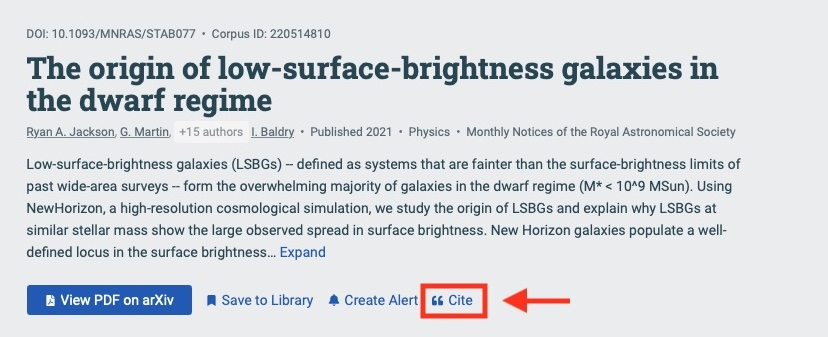
\includegraphics[width=0.8\hsize]{bib-1.jpg}\\[2mm]
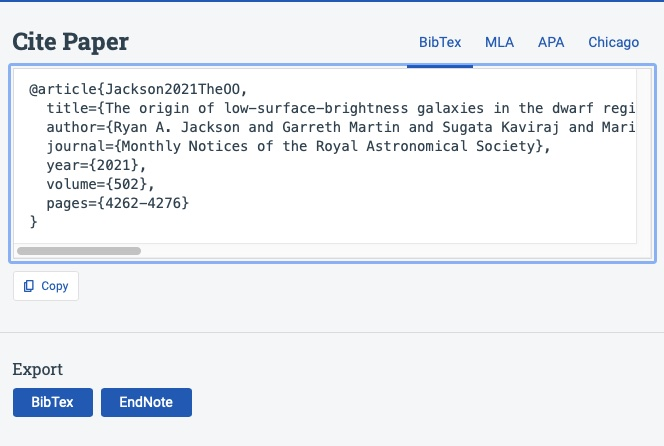
\includegraphics[width=0.8\hsize]{bib-2.jpg}\\[2mm]
\caption{Пример экспорта Bib\TeX-файла на примере системы SemanticScholar}\label{fig:BibTex}
\end{center}
\end{figure}

\newpage
\textbf{ВНИМАНИЕ!}

К списку источников предьявляютя особые требования. Это касается как его
содержания, так и количества источников, на которые вы ссылаетесь в своем
отчете. В первой строке таблицы~\ref{tab:lit} указан номер курса, для
которого в строке ниже приведено минимальное общее количество источников,
на которые есть ссылки в работе. В последующих строках приведено минимальное
количество источников разных типов. Под научно-периодической литературой
подразумевается наличие ссылок на статьи в периодических тематических журналах.

\begin{table}[h]
\caption{Название таблицы. Таблицы следует размещать в основном тексте рядом с первым цитированием.}
\label{tab:lit}
\begin{center}
\begin{tabular}{|p{7.5 cm}|c|c|c|c|c|}
\hline
 Номер курса & 2 & 3 & 4 & 5 & 6\\
\hline
Общее количество используемой литературы из них: & > 15 & > 20 & > 25 & > 30 & > 30 \\
\hline
- на иностранных языках & $\ge$4 & $\ge$5 & $\ge$6 & $\ge$7 & $\ge$7 \\
\hline
- текущая научно-периодическая литература (после 2010 г.)& $\ge$3 & $\ge$5 & $\ge$7 & $\ge$7 & $\ge$7  \\
\hline
- литература 21 века & $\ge$10 & $\ge$15 & $\ge$21 & $\ge$21 & $\ge$21 \\
\hline
\end{tabular}
\end{center}
\end{table}
